


\section{Additional Dataset Information}\label{app:datasets}
In Table \ref{fig:dataset} we provide further dataset-specific information on the BEIR retrieval datasets used in this paper. Specifically, we state the sizes of the query and corpuses used, as well as the average number of embeddings produced by the ColBERTv2 model per document. Specifically, we consider the six BEIR retrieval datasets MS MARCO \cite{nguyen2016ms},
NQ \cite{kwiatkowski2019natural},
HotpotQA \cite{yang2018hotpotqa},
ArguAna \cite{wachsmuth2018retrieval},
SciDocs \cite{cohan2020specter},  and
Quora \cite{thakur2021beir}, Note that the MV corpus (after generating MV embeddings on all documents in a corpus) will have a total of $\#$Corpus $\times$ (Avg $\#$ Embeddings per Doc) token embeddings. 
For even further details, see the BEIR paper \cite{thakur2021beir}. 



\begin{figure}[h]
    \centering
    \begin{tabular}{|c|c|c|c|c|c|c|} % Vertical lines before, between, and after columns
\hline % HorMS MARCO	ArguAna	SciDocs	NQ	Quora	HotpotQAizontal line after the first row
& MS MARCO & HotpotQA & NQ  & Quora & SciDocs &  ArguAna \\ \hline
$\#$Queries & 6,980 &7,405 & 3,452& 10,000 &1,000 &  1,406 \\ \hline
$\#$Corpus &8.84M & 5.23M &  2.68M  &523K & 25.6K  & 8.6K  \\\hline
\makecell{Avg \\$\#$ Embeddings\\ per Doc}
 & 78.8&	68.65&	100.3 & 18.28 &	165.05 &	154.72 \\\hline
 % Horizontal line at the bottom
\end{tabular}
    \caption{Dataset Specific Statistics for the BEIR datasets considered in this paper. }
    \label{fig:dataset}
\end{figure}

\section{Additional Experiments and Plots} \label{sec:additional-plots}
In this Section, we provide additional plots to support the experimental results from Section \ref{sec:eval}. We providing plots for all six of the datasets and additional ranges of the $x$-axis for our experiments in Section (§\ref{sec:fde-experimental}), as well as additional experimental results, such as an evaluation of variance, and of the quality of final projections in the FDEs. 

\paragraph{FDE vs. SV Heuristic Experiments.} In Figures \ref{fig:sv_mv_full5k} and \ref{fig:sv_mv_full500}, we show further datasets and an expanded recall range for the comparison of the SV Heuristic to retrieval via FDEs. We find that our 4k+ dimensional FDE methods outperform even the deduplciated SV heuristic (whose cost is somewhat unrealistic, since the SV heuristic must over-retrieve to handle duplicates) on most datasets, especially in lower recall regimes. 
In Table \ref{table:sv_mv_table}, we compare how many candidates must be retrieved by the SV heuristic, both with and without the deduplciation step, as well as by our FDE methods, in order to exceed a given recall threshold. 


\begin{table}[h!]
    \centering
    \begin{tabular}{|c|c|c|c|c|c|c|} \hline
\makecell{Recall\\ Threshold} &SV non-dedup  & SV dedup & 20k FDE & 10k FDE &4k FDE&  2k FDE  \\ \hline
80\% & 1200 & 300 & 60 & 60& 80 & 200\\  \hline
85\% & 2100 & 400&  90 & 100 & 200& 300 \\  \hline
90\% &4500 & 800& 200 & 200& 300 &  800 \\ \hline
95\% & >10000& 2100 & 700 &800  & 1200 & 5600 \\ \hline 
\end{tabular}
\vspace{1em}
  \caption{FDE retrieval vs SV Heuristic: number of candidates that must be retrieved by each method to exceed a given recall on MS MARCO. The first two columns are for the SV non-deduplicated and deduplicated heuristics, respectively, and the remaining four columns are for the FDE retrieved candidates with FDE dimensions $\{20480,10240,4096,2048\}$, respectively. Recall$@N$ values were computed in increments of $10$ between $10$-$100$, and in increments of $100$ between $100$-$10000$, and were not computed above $N > 10000$.  } 
    \label{table:sv_mv_table}
\end{table}


\paragraph{Retrieval quality with respect to exact Chamfer.} In Figure \ref{fig:mv_vs_bf_full}, we display the full plots for FDE Recall with respects to recovering the $1$-nearest neighbor under Chamfer Similarity for all six BEIR datasets that we consider, including the two omitted from the main text (namely, SciDocs and ArguAna). 



\subsection{Variance of FDEs.} \label{app:variance} Since the FDE generation is a randomized process, one natural concern is whether there is large variance in the recall quality across different random seeds. Fortunately, we show that this is not the case, and the variance of the recall of FDE is essentially negligible, and can be easily accounted for via minor extra retrieval. To evaluate this, we chose four sets of FDE parameters $(\reps,\ksim,\dproj)$ which were Pareto optimal for their respective dimensionalities, generated $10$ independent copies of the query and document FDEs for the entire MS MARCO dataset, and computed the average recall$@100$ and $1000$ and standard deviation of these recalls. The results are shown in Table \ref{fig:variance}, where for all of the experiments the standard deviation was between $0.08$-$0.3\%$ of a recall point, compared to the $~80$-$95\%$ range of recall values. Note that Recall$@1000$ had roughly twice as small standard deviation as Recall$@$100.

\begin{table}[h!]
    \centering
    \begin{tabular}{|c|c|c|c|c|} % Vertical lines before, between, and after columns
\hline 
FDE params $(\reps,\ksim,\dproj)$ &$(20,5,32)$ &  $(20,5,16)$& $(20,  4,16)$ & $(20,4,8)$ \\ % First row
\hline % Horizontal line after the first row
FDE Dimension & 20480 & 10240 & 5120 & 2560 \\
\hline
 Recall@100  & 83.68 & 82.82	&80.46 &	77.75 \\ % Second row (empty cells)
Standard Deviation & 0.19&	0.27	& 0.29&	0.17\\ % Third row (empty cells)
\hline
Recall@1000  & 95.37 & 94.88 & 93.67 & 91.85  \\ % Second row (empty cells)
Standard Deviation & 0.08 & 0.11 & 0.16 & 0.12  \\ % Third row (empty cells)
\hline % Horizontal line at the bottom
\end{tabular}
\vspace{1em}
  \caption{Variance of FDE Recall Quality on MS MARCO.  }
    \label{fig:variance}
\end{table}

%%%%%%%%%%%%%%%%%%%%%%%%%%%%%%%%



\newpage
\begin{figure}[t]
    \centering
  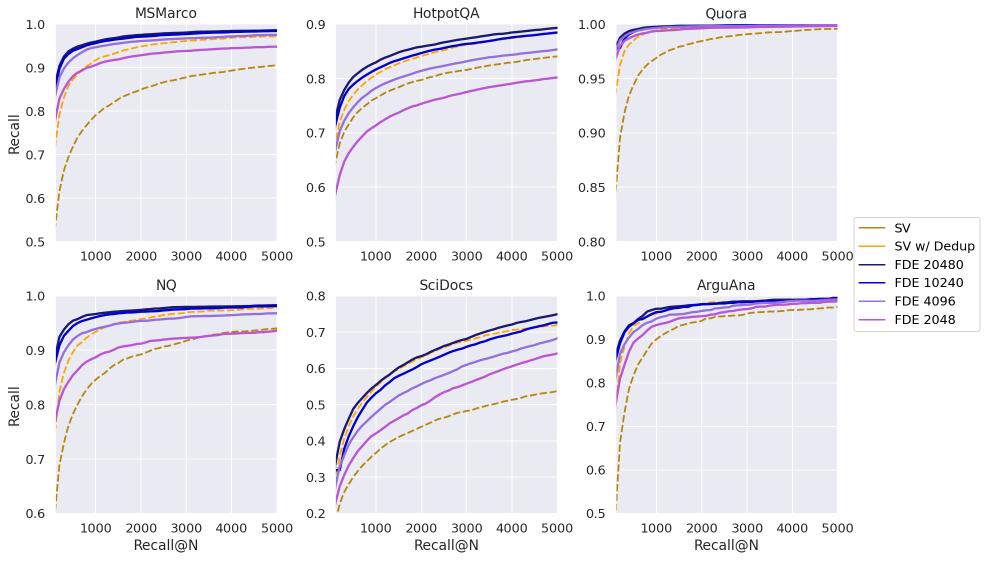
\includegraphics[width=\linewidth]{plots/SV_vs_MV_full5k_v2.png}
   \caption{FDE retrieval vs SV Heuristic, Recall$@100$-$5000$}
         \label{fig:sv_mv_full5k} % Add a label (optional)
\end{figure}

\begin{figure}[t]
    \centering
  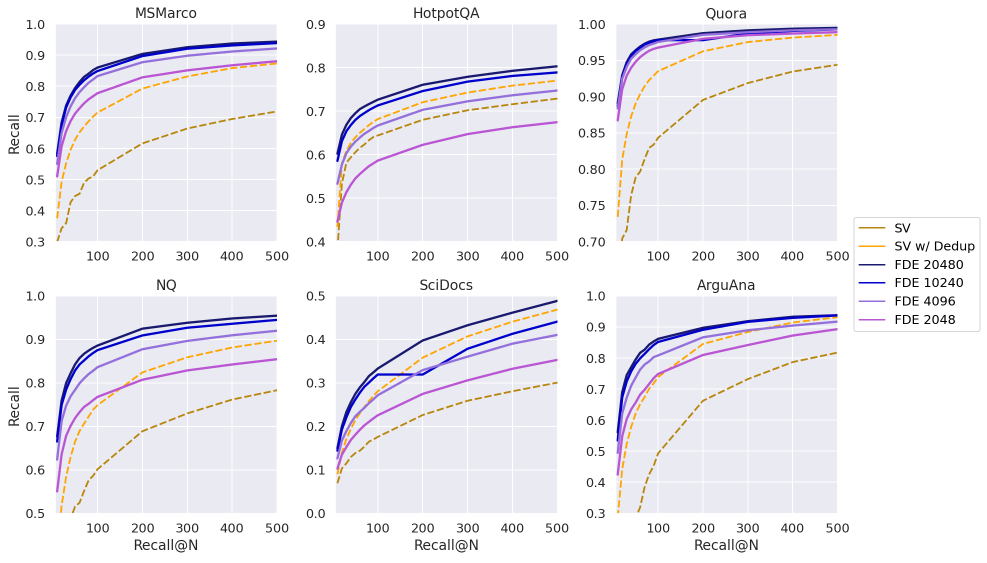
\includegraphics[width=\linewidth]{plots/SV_vs_MV_full500_v2.png}
   \caption{FDE retrieval vs SV Heuristic, Recall$@5$-$500$}
         \label{fig:sv_mv_full500} % Add a label (optional)
\end{figure}



\begin{figure}[h!]
    \centering
  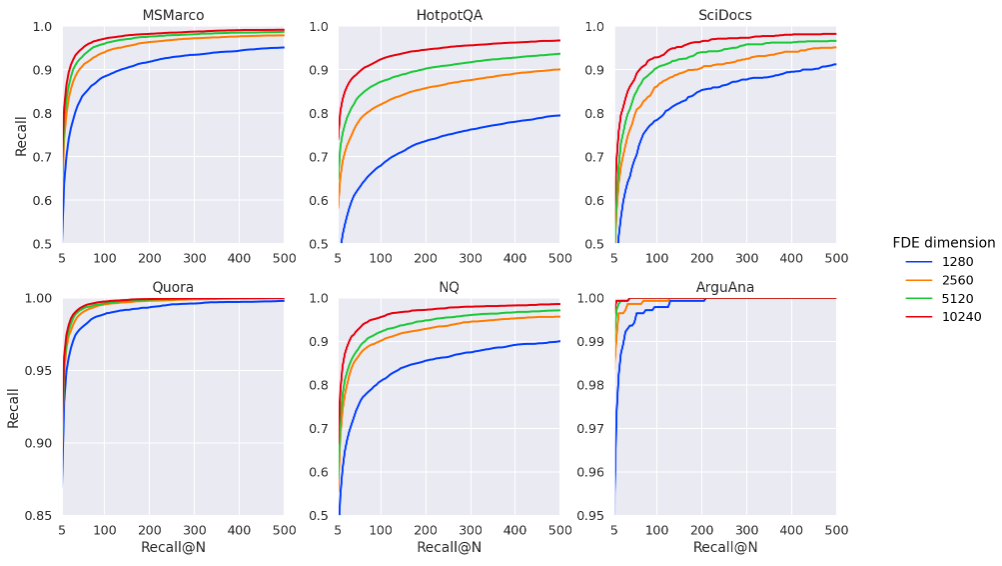
\includegraphics[width=\linewidth]{plots/MV_vs_bruteforce_v2.png}
    \caption{Comparison of FDE recall with respect to the most similar point under Chamfer.}
          \label{fig:mv_vs_bf_full} % Add a label (optional)
\end{figure}



\begin{table}[h!]
    \centering
    \begin{tabular}{c|c c | c c | }\hline
        Experiment & w/o projection & w/ projection &  w/o projection & w/ projection \\\hline
      % Experiment &  (20,5,8) &(40,6,128) w/ projection & (20,5,16) &(40,6,128) w/ projection  \\\hline
      Dimension  & 2460& 2460& 5120& 5120 \\\hline
      Recall@100  & 77.71 & 78.82 &80.37 & 83.35 \\\hline
      Recall@1000  & 91.91 & 91.62 & 93.55 & 94.83 \\\hline
         Recall@10000  &97.52 & 96.64 & 98.07 & 98.33 \\\hline
    \end{tabular}
    \vspace{1em}
    \caption{Recall Quality of Final Projection based FDEs with $\dfde \in \{2460,5120\}$}
    \label{tab:finalproj1}
\end{table}



\begin{table}[h!]
    \centering
    \begin{tabular}{c|c c | c c | }\hline
        Experiment & w/o projection & w/ projection &  w/o projection & w/ projection \\\hline
      % Experiment &  (20,5,8) &(40,6,128) w/ projection & (20,5,16) &(40,6,128) w/ projection  \\\hline
      Dimension  & 10240& 10240& 20480& 20480 \\\hline
      Recall@100  &82.31 & 85.15 & 83.36 & 86.00 \\\hline
      Recall@1000  & 94.91 & 95.68 & 95.58 & 95.95 \\\hline
         Recall@10000  &98.76 & 98.93 & 98.95 & 99.17\\\hline
    \end{tabular}
    \vspace{1em}
      \caption{Recall Quality of Final Projection based FDEs with $\dfde \in \{10240,20480\}$}
       \label{tab:finalproj2}
\end{table}

\newpage

\subsection{Comparison to Final Projections.} \label{app:finalproj}
We now show the effect of employing final projections to reduce the target dimensionality of the FDE's. For all experiments, the final projection $\bpsi'$ is implemented in the same way as inner projections are: namely, via multiplication by a random $\pm 1$ matrix. 
We choose four target dimensions, $\dfde \in \{2460,5120,10240,20480\}$, and choose the Pareto optimal parameters $(\reps, \ksim, \dproj)$ from the grid search without final projections in Section \ref{sec:fde-experimental}, which are $(20,4,8),(20,5,8),(20,5,16),(20,5,32)$. We then build a large dimensional FDE with the parameters $(\reps,\ksim,\dproj) = (40,6,128)$. Here, since $d = \dproj$, we do not use any inner productions when constructing the FDE. We then use a single random final projection to reduce the dimensionality of this FDE from $\reps \cdot 2^{\ksim} \cdot \dproj = 327680$ down to each of the above target dimensions $\dfde$. The results are show in Tables \ref{tab:finalproj1} and \ref{tab:finalproj2}. Notice that incorporating final projections can have a non-trivial impact on recall, especially for Recall$@$100, where it can increase by around $3\%$. In particular, FDEs with the final projections are often better than FDEs with twice the dimensionality without final projections. The one exception is the  $2460$-dimensional FDE, where the Recall$@$100 only improved by $1.1\%$, and the Recall$@$1000 was actually lower bound $0.3\%$.

